
%% single column for submission and review
%\documentclass[journal, onecolumn, 12pt, a4paper, draftcls]{IEEEtran}

%% double column to emulate final version (for submission and review)
\documentclass[10pt, twocolumn, twoside]{IEEEtran}

%% double column for conference
%\documentclass[conference]{IEEEtran}

\IEEEoverridecommandlockouts
\bibliographystyle{IEEEtran}

\usepackage[cmex10]{amsmath} % prevents amsmath from using a Type 3 font for math within footnotes
\interdisplaylinepenalty=2500 % (re)allows page breaks within aligned equations
\usepackage{amssymb}
\usepackage{bm}
\usepackage{mathtools}
\usepackage{cite}
\usepackage{xcolor}
\usepackage{enumerate}
\usepackage{booktabs} % nice table objects
\usepackage{multirow}
\usepackage{lipsum}
\usepackage{graphicx}
\usepackage{breqn}

\graphicspath{{figs/}{pdf/}{jpg/}{../pdf/}}

%commands
%\renewcommand{\phi}{\varphi}
\newcommand{\untsph}{\mathbb{S}^{2}} % unit sphere
\newcommand{\unit}[1]{\widehat{\bm{#1}}}
\DeclarePairedDelimiterX\abs[1]{\lvert}{\rvert}{#1}
\DeclarePairedDelimiterX\parn[1]{(}{)}{#1}
\DeclarePairedDelimiterX\set[1]{\lbrace}{\rbrace}{#1}
\DeclarePairedDelimiterX\innerp[2]{\langle}{\rangle}{#1,#2}
\DeclarePairedDelimiterX\norm[1]{\lVert}{\rVert}{#1}
\DeclarePairedDelimiterX\brak[1]{\lbrace}{\rbrace}{#1}
\DeclareMathOperator{\expectop}{\mathbb{E}} % \expect[\Big]{ f }
\newcommand{\expect}[2][]{\expectop\brak[#1]{#2}}

\newcommand{\figref}[1]{Fig.\,\ref{#1}}
\newcommand{\tabref}[1]{Table~\ref{#1}}
\newcommand{\reals}{\mathbb{R}} % real numbers
\newcommand{\cmplx}{\mathbb{C}} % complex numbers
\newcommand{\dfn}{\triangleq}
\newcommand{\conj}[1]{\overline{#1}} % conjugate
\newcommand{\tendsto}{\rightarrow}

\newtheorem{theorem}{Theorem}%[section]
\renewcommand{\IEEEQED}{\IEEEQEDopen}

\begin{document}

\title{Robust Slepian Functions on the Sphere}

\ifCLASSOPTIONconference
	\author{
		\IEEEauthorblockN{Rodney~A.~Kennedy}
			\thanks{This research was supported under the Australian Research Council's Discovery Projects
				funding scheme (Project No.~DP1094350).}
		\IEEEauthorblockA{Research School of Engineering,\\
			College of Engineering and Computer Science,\\
			The Australian National University,\\ Canberra, ACT 0200, Australia\\
			Email: rodney.kennedy@anu.edu.au} \and
		\IEEEauthorblockN{Collaborator}
		\IEEEauthorblockA{Research School of Engineering,\\
			College of Engineering and Computer Science,\\
			The Australian National University,\\ Canberra, ACT 0200, Australia\\
			Email: collaborator@anu.edu.au}}
\else
	\author{Rodney~A.~Kennedy,~\IEEEmembership{Fellow,~IEEE}, and
		Collaborator,~\IEEEmembership{Senior Member,~IEEE}
		\thanks{Rodney~A.~Kennedy and Collaborator are with the Research School of Engineering,
			College of Engineering and Computer Science,
			The Australian National University (ANU), Canberra, ACT 0200, Australia
			(email: $\{$rodney.kennedy, collaborator$\}$@anu.edu.au).}
		\thanks{This work was supported under the Australian Research Council's Discovery Projects
			funding scheme (Project No.~DP1094350).}}
\fi


\maketitle


\begin{abstract}
Slepian functions on the sphere maximally concentrate energy inside a region for a given bandlimit.
\end{abstract}

\smallskip
\begin{IEEEkeywords}
key, word, keyword list
\end{IEEEkeywords}

\IEEEpeerreviewmaketitle

\section{Introduction}

\subsection{Background}

\lipsum[4-6]  The most profound work is found in\cite{Kennedy-book:2013}.

%\begin{figure}
%\centering
%	\includegraphics[width=0.59\columnwidth]{pdfs/xxx1.png}\\
%	\caption{Description}\label{fig:nice-fig}
%\end{figure}

\subsection{Contributions}

$\expect{f}$ and $\expect[\big]{f}$

\begin{itemize}
\item
\lipsum[17]
\item
\lipsum[18]
\item
\lipsum[19]
\end{itemize}


%\lipsum[33-36]

\newpage

\section{Problem Formulation}

\subsection{Notation}

The natural Hilbert space on the sphere is denoted $L^2(\untsph)$ with inner product
\(
	\innerp{f}{g}\dfn\int_{\untsph} f(\unit{x})\,
		\conj{g(\unit{x})}\,ds(\unit{x}).
\)
The spherical harmonic transform (SHT) is given by
\[
	(f)_{\ell}^{m}=\innerp[\big]{f}{Y_{\ell}^{m}}
	=\int_{\untsph} f(\unit{x})\,\conj{Y_{\ell}^{m}(\unit{x})}\,ds(\unit{x})
\]
for degree $\ell\in\set{0,1,\dots}$ and order $m$ where $\abs{m}\leq \ell$.

The subspace of band-limited functions on the sphere of maximum degree $L$ is denoted $\mathcal{H}_{L}\in L^2(\untsph)$ and is $N\dfn(L+1)^2$-dimensional.  If a signal $f(\unit{x})$ is band-limited to $L$ then $\innerp{f}{Y_{\ell}^{m}}=0$ for $\ell>L$ and it has the spectral (spherical harmonic) representation given by the vector
\begin{equation}
\label{eqn:f-spec}
	\mathbf{f}=\parn[\Big]{(f)_0^0, (f)_1^{-1}, (f)_1^{0}, (f)_1^{1},\dotsc, (f)_L^{L}}
	\in\cmplx^{N}.
\end{equation}
This vector can be indexed with $n=0,1,2,\dotsc,N-1$, where $n=\ell(\ell+1)+m$.  Generally when we say $f$ is band-limited then the maximum degree $L$ is understand.

The spatial and spectral representations are related through isomorphism\cite{Kennedy-book:2013}
\begin{equation}
\label{eqn:isom}
	\innerp{f}{g}=\innerp{\mathbf{f}}{\mathbf{g}}_{\cmplx^N},
\end{equation}
where the spectral inner product is $\innerp{\mathbf{f}}{\mathbf{g}}=\mathbf{g}^H\mathbf{f}$.
This isomorphism greatly simplifies our demonstrations of different types of orthogonality.

\subsection{Weighted spatial concentration problem}

Let $h(\unit{x})$ be a real, non-negative weighting function bounded by unity on the unit sphere $\untsph$.  Then we seek the band-limited signal $f(\unit{x})\in\mathcal{H}_{L}$ that maximizes the following weighted spatial concentration
\begin{equation}
\label{eqn:conc-spat}
	\lambda_0
		=\max_{f\in\mathcal{H}_{L}}
		\set[\Bigg]{\frac{\int_{\untsph} h(\unit{x})\,\abs[\big]{f(\unit{x})}^2\,ds(\unit{x})}%
		{\int_{\untsph} \abs[\big]{f(\unit{x})}^2\,ds(\unit{x})}}.
\end{equation}
The denominator in \eqref{eqn:conc-spat} can be written $\norm{f}^2$ and is usually taken to be unity.

The weighted concentration problem \eqref{eqn:conc-spat} can be written in the spectral domain as the Rayleigh quotient
\begin{equation}
\label{eqn:conc-spec}
	\lambda_0
		=\max_{\mathbf{f}\in\cmplx^{H}}\frac{\mathbf{f}^H\mathbf{H}\mathbf{f}}%
		{\mathbf{f}^H\mathbf{f}},
\end{equation}
where the spectral Hermitian matrix $\mathbf{H}$ has elements
\begin{equation}
\label{eqn:W-matrix}
	H_{\ell,p}^{m,q} \dfn \int_{\untsph} h(\unit{x})\,Y_{p}^{q}(\unit{x})\,
		\conj{Y_{\ell}^{m}(\unit{x})}\,ds(\unit{x}),
\end{equation}
and $\mathbf{f}$ is the spectral representation of $f(\unit{x})$.  Note that the rows and columns of matrix $\mathbf{H}$ are indexed consistent with $\mathbf{f}$ in \eqref{eqn:f-spec}.

Problem \eqref{eqn:conc-spec} is solved by finding the eigenvector corresponding to the largest eigenvalue of $\mathbf{H}$.  All eigenvalues of $\mathbf{H}$ are real and non-negative, $\lambda_0\geq\lambda_1\geq\lambda_2\geq\dotsb\geq0$, and the corresponding eigenvectors, $\mathbf{v}_0,\mathbf{v}_1, \mathbf{v}_2, \dotsc,$ can be chosen as orthonormal.  If the components of the dominant spectral eigenvector, $\mathbf{v}_0$, are $(v^{}_0)_{\ell}^{m}$ then the spatial eigen-function is
\begin{align}
\label{eqn:spat-eigen}
	v^{}_{0}(\unit{x})
	&=\smash{\sum_{\ell,m}} (v^{}_0)_{\ell}^{m}\, Y_{\ell}^{m}(\unit{x}) \\
	&=\arg\max_{f\in\mathcal{H}_{L}}
		\set[\Bigg]{\frac{\int_{\untsph} h(\unit{x})\,\abs[\big]{f(\unit{x})}^2\,ds(\unit{x})}%
		{\int_{\untsph} \abs[\big]{f(\unit{x})}^2\,ds(\unit{x})}}. \nonumber
\end{align}
In summary, to find the optimal spatial function that attains \eqref{eqn:conc-spat}, being $v_{0}(\unit{x})$ in \eqref{eqn:spat-eigen}, we compute the spectral Hermitian matrix, using \eqref{eqn:W-matrix}; then determine the dominant spectral eigenvector $\mathbf{v}_0$; and synthesize $v_{0}(\unit{x})$ using the inverse SHT in \eqref{eqn:spat-eigen}.

%\subsection{Slepian spatial concentration}
%
%Defining a region $R\in\untsph$, then selecting the real, non-negative weighting function, $h(\unit{x})$, as
%\begin{equation}
%\label{eqn:indicator}
%	\chi^{}_{R}(\unit{x}) \dfn
%	\begin{cases}
%		1 & \unit{x}\in R \\
%		0 & \text{otherwise}
%	\end{cases},
%\end{equation}
%then we recover the standard Slepian concentration problem on the sphere
%\begin{equation}
%\label{eqn:conc-spat-slep}
%	\lambda_0
%		=\max_{f\in\mathcal{H}_{L}}\frac{\int_{R} \abs[\big]{f(\unit{x})}^2\,ds(\unit{x})}%
%		{\int_{\untsph} \abs[\big]{f(\unit{x})}^2\,ds(\unit{x})},
%\end{equation}
%whose spectral Hermitian matrix $\mathbf{H}$ has elements
%\begin{equation}
%\label{eqn:W-matrix-slep}
%	H_{\ell,p}^{m,q} \dfn \int_{R} Y_{p}^{q}(\unit{x})\,
%		\conj{Y_{\ell}^{m}(\unit{x})}\,ds(\unit{x}).
%\end{equation}
%Then $\mathbf{H}\mathbf{v}_0=\lambda_0\mathbf{v}_0$, and $\mathbf{v}_0$ is the spectral representation of the most concentrated signal, as synthesized in \eqref{eqn:spat-eigen}.
%
%For illustration, let the region $R\in\untsph$ be the Australian continent including Tasmania, and let band-limit $L=20$.  The resulting spectral Hermitian matrix $\mathbf{H}$ is $441\times441$. The two dominant eigen-functions $v^{}_{0}(\unit{x})$ and $v^{}_{1}(\unit{x})$ are shown in Fig.\,\ref{fig:region}.

\subsection{Three-fold spatial orthogonality of eigen-functions}

Firstly, with the $N$ eigenvectors $\mathbf{v}_n$, $n=0,1,2,\dotsc,N-1$, of $\mathbf{H}$ are orthonormal in $\cmplx^N$.  Then by isomorphism, \eqref{eqn:isom}, we have \emph{orthonormality} of the $N$ eigen-functions $v_n(\unit{x})$ in $\mathcal{H}_{L}$.  That is, from \eqref{eqn:isom},
\[
	\innerp{v_n(\unit{x})}{v_m(\unit{x})}
	=\innerp{\mathbf{v}_n}{\mathbf{v}_m}_{\cmplx^N}
	=\delta_{m,n}.
\]

Secondly, spectrally (because we have eigenvectors) then
\begin{align*}
	\innerp{\mathbf{H}\mathbf{v}_n}{\mathbf{v}_m}_{\cmplx^N}
	=\mathbf{v}_m^H\mathbf{H}\mathbf{v}_n
	&=\mathbf{v}_m^H\lambda_n\mathbf{v}_n \\
	&=\lambda_n\innerp{\mathbf{v}_n}{\mathbf{v}_m}_{\cmplx^N}
	=\lambda_n\,\delta_{n,m}.
\end{align*}
So, by isomorphism, spatially this is the same as
\[
	\int_{\untsph} h(\unit{x})\,v_n(\unit{x})\,
		\conj{v_m(\unit{x})}\,ds(\unit{x})=\lambda_n\,\delta_{n,m}.
\]
This is spatial \emph{orthogonality} of the $v_n(\unit{x})$ with respect to a weighted spatial inner product on the sphere
\[
	\innerp{f}{g}_{h}\dfn\int_{\untsph} h(\unit{x})\,f(\unit{x})\,
		\conj{g(\unit{x})}\,ds(\unit{x}).
\]
Under this weighted inner product $\norm{v_n(\unit{x})}^2_{h}=\lambda_n$, which is less than unity in general.  However, it is clear that, whenever $\lambda_n>0$,
\[
	\set[\Big]{\frac{1}{\sqrt{\lambda_n}}v_n(\unit{x})}
\]
are \emph{orthonormal} in the weighted inner product space.

Finally, there is a third sense in which the $v_n(\unit{x})$ are orthogonal.  Implicitly define a third inner product through
\[
	\innerp{f}{g}=\innerp{f}{g}_{h}+\innerp{f}{g}_{1-h}.
\]
Then given $0\leq h(\unit{x})\leq1$ we have $0\leq1-h(\unit{x})\leq1$ and $v_n(\unit{x})$ are also \emph{orthogonal} in the complementary weighted inner product space
\[
	\innerp{f}{g}_{1-h}\dfn\int_{\untsph} \parn[\Big]{1-h(\unit{x})}\,f(\unit{x})\,
		\conj{g(\unit{x})}\,ds(\unit{x}),
\]
and can be normalized in an expected way ($\lambda_n<1$)
\[
	\set[\Big]{\frac{1}{\sqrt{1-\lambda_n}}v_n(\unit{x})}.
\]
Further, in this case, the Hermitian matrix is $\mathbf{H}^{c}\dfn\mathbf{I}-\mathbf{H}$.

In summary, the eigenfunctions satisfy the three-fold \emph{spatial orthogonality} (with spectral counterparts):
\begin{align*}
	\innerp{v_n(\unit{x})}{v_m(\unit{x})}&=\delta_{m,n}
		&&(= \innerp{\mathbf{v}_n}{\mathbf{v}_m}_{\cmplx^N})\\
	\innerp{v_n(\unit{x})}{v_m(\unit{x})}_h&=\lambda_n\,\delta_{m,n}
		&&(=\innerp{\mathbf{H}\mathbf{v}_n}{\mathbf{v}_m}_{\cmplx^N})\\
	\innerp{v_n(\unit{x})}{v_m(\unit{x})}_{1-h}&=(1-\lambda_n)\,\delta_{m,n}
		&&(=\innerp{\mathbf{H}^{c}\mathbf{v}_n}{\mathbf{v}_m}_{\cmplx^N})
\end{align*}
which implies the energy concentrations are $\norm{v_n(\unit{x})}^2=1$, $\norm{v_n(\unit{x})}_h^2=\lambda_n$, and $\norm{v_n(\unit{x})}_{1-h}^2=1-\lambda_n$.

\subsection{Slepian spatial concentration}

Defining a region $R\in\untsph$, then selecting the real, non-negative weighting function, $h(\unit{x})$, as
\begin{equation}
\label{eqn:indicator}
	\chi^{}_{R}(\unit{x}) \dfn
	\begin{cases}
		1 & \unit{x}\in R \\
		0 & \text{otherwise}
	\end{cases},
\end{equation}
then we recover the standard Slepian concentration problem on the sphere\cite{Kennedy-book:2013}
\begin{equation}
\label{eqn:conc-spat-slep}
	\lambda_0
		=\max_{f\in\mathcal{H}_{L}}\frac{\int_{R} \abs[\big]{f(\unit{x})}^2\,ds(\unit{x})}%
		{\int_{\untsph} \abs[\big]{f(\unit{x})}^2\,ds(\unit{x})},
\end{equation}
whose spectral Hermitian matrix $\mathbf{H}$ has elements
\begin{equation}
\label{eqn:W-matrix-slep}
	H_{\ell,p}^{m,q} \dfn \int_{R} Y_{p}^{q}(\unit{x})\,
		\conj{Y_{\ell}^{m}(\unit{x})}\,ds(\unit{x}).
\end{equation}
Then $\mathbf{H}\mathbf{v}_0=\lambda_0\mathbf{v}_0$, and $\mathbf{v}_0$ is the spectral representation of the most concentrated signal, as synthesized in \eqref{eqn:spat-eigen}.

We have the three-fold spatial orthogonality of Slepian eigen-functions.  They are orthonormal on the whole sphere, orthogonal within region $R$ and orthogonal within region $\untsph\setminus{}R$.
Within the regions (subregions of the sphere) the effective inner product weighting is unity, that is,
\begin{align*}
	\innerp{f}{g}_{h} 
		&=\int_{R} f(\unit{x})\,\conj{g(\unit{x})}\,ds(\unit{x}), \\
		\shortintertext{and}
	\innerp{f}{g}_{1-h} 
		&=\int_{\untsph\setminus{}R} f(\unit{x})\,\conj{g(\unit{x})}\,ds(\unit{x}).
\end{align*}

For illustration, on the Earth, normalized with unit radius, let the region $R\in\untsph$ be the Australian continent including Tasmania, and let band-limit $L=20$.  The resulting spectral Hermitian matrix $\mathbf{H}$ is $441\times441$. The two dominant eigen-functions $v^{}_{0}(\unit{x})$ and $v^{}_{1}(\unit{x})$ are shown in Fig.\,\ref{fig:region}.

\begin{figure}[htb]
\centering
	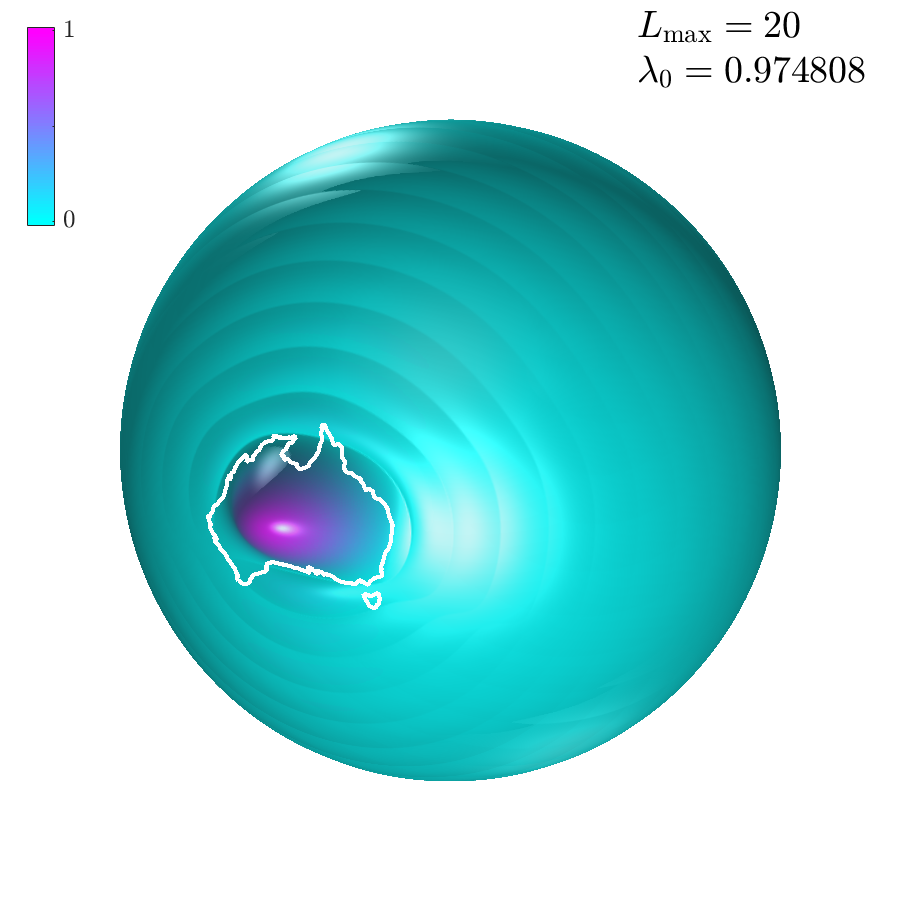
\includegraphics[width=0.65\columnwidth]{pdfs/australia_0020_0001.png}\\[-5mm]
	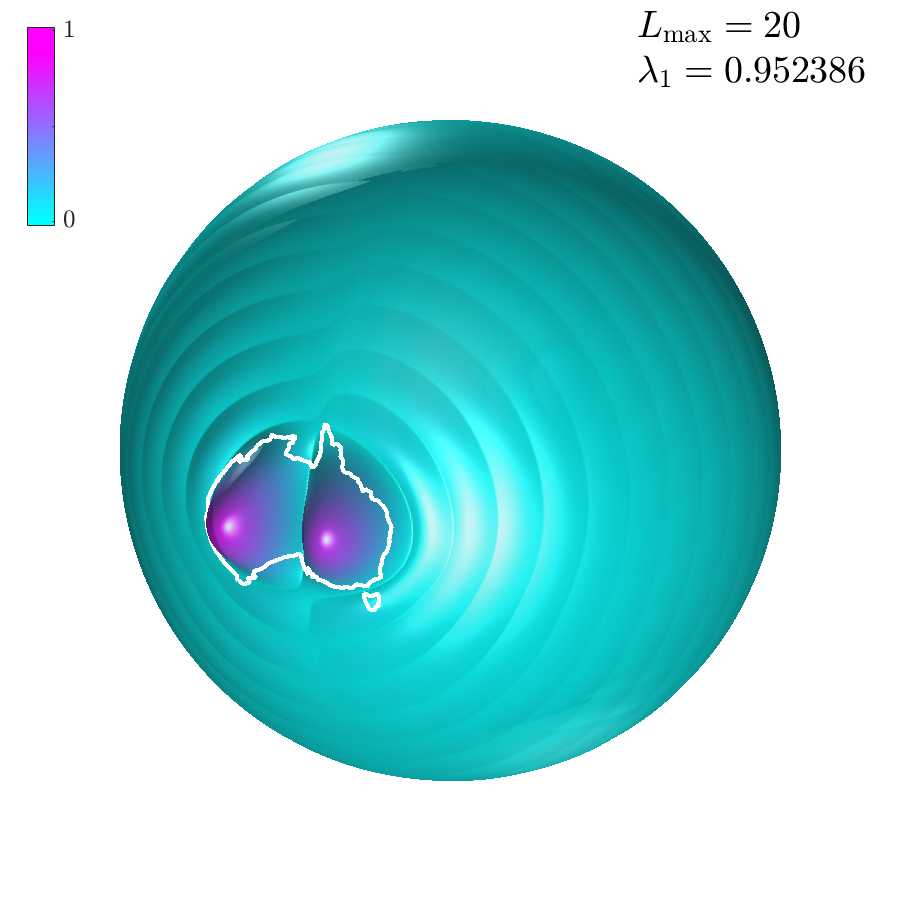
\includegraphics[width=0.65\columnwidth]{pdfs/australia_0020_0002.png}
	\caption{The two dominant eigen-functions $v^{}_{0}(\unit{x})$ and $v^{}_{1}(\unit{x})$ for Australia including Tasmania for band-limit $L=20$.}\label{fig:region}
\end{figure}


\quad
\newpage

\section{Dummy}

\begin{theorem}[Kennedy's Lemon]
\label{thm:main}
\lipsum[46]
\end{theorem}

\medskip

\begin{IEEEproof}
\lipsum[47]
\end{IEEEproof}

\begin{table}[tbp]
\renewcommand{\arraystretch}{1.0}
\caption{Model parameters in the general form}
\begin{center}
	\begin{tabular}{@{\,}cccc@{\,}}
		\toprule
			\multirow{2}{*}{\bfseries Model} & \multirow{2}{*}{\bfseries Expansion}
				& \bfseries Coefficients & \bfseries Weighting \\
			& & $\displaystyle\iota_{n;q}^{m}$ & $g_{n}(k,r)$ \\[1mm]
		\midrule
			1 & Source Distribution & $\gamma_{n;q}^{m}$
				& $ik\, j_{n}(ks) h_{n}^{(1)}(kr)$ \\[0.8mm]
			2 & Radiating Solution & $\zeta_{n;q}^{m}$
				& $h_{n}^{(1)}(kr)$ \\[0.8mm]
			3 & Nominal Radius& $\rho_{n;q}^{m[r_{0}]}$
				& $h_{n}^{(1)}(kr)/h_{n}^{(1)}(kr_{0})$ \\[1mm]
		\bottomrule
	\end{tabular}
\end{center}
\label{tab:models}
\end{table}

\newskip\conditionsep
\conditionsep=10pt minus5pt


Equation example
\ifCLASSOPTIONtwocolumn
\begin{multline}
	\iota_{n;q}^{m} = 4\sqrt{1-\pi^{2}}
		\int_{0}^{\mathrlap{k_{u}}\;}
		\frac{1}{g_{n}(k,r_{1})}
		\times \\
	\int_{\untsph} H(r_{1},\unit{x};k)
		\conj{Y_{n}^{m}(\unit{x})}\,ds(\unit{x})\, \conj{\varphi_{q}(k)}\,dk.
\end{multline}
\else
\begin{subequations}
\begin{equation}
	\iota_{n;q}^{m} = 4\sqrt{1-\pi^{2}}
		\int_{0}^{\mathrlap{k_{u}}\;}
		\frac{1}{g_{n}(k,r_{1})} 
	\int_{\untsph} H(r_{1},\unit{x};k)
		\conj{Y_{n}^{m}(\unit{x})}\,ds(\unit{x})\, \conj{\varphi_{q}(k)}\,dk,\quad r_1>a.
\end{equation}
\end{subequations}
\fi
or using the {\tt breqn} package
\begin{dmath}
	\iota_{n;q}^{m} = 4\pi
		\int_{0}^{\mathrlap{k_{u}}\;}
		\frac{1}{g_{n}(k,r_{1})} \times
	\int_{\untsph} H(r_{1},\unit{x};k)
		\conj{Y_{n}^{m}(\unit{x})}\,ds(\unit{x})\, \conj{\varphi_{q}(k)}\,dk%\condition{for $r_1>a$}.
\end{dmath}


\section{Conclusions}

\lipsum[28]

\bibliography{IEEEabrv,xxx}

\appendices

\section{Obscure Thing}

\lipsum[38]

\section{Unclear Thing}

\lipsum[39-41]

\end{document}



